\vspace{2ex}

    {\bf Solution.} I shall verify the likelihood of the model is identifiable
    and it brings the information from the data to the parameter. I say a
    model is identifiable if the implication 
    $$P_{\theta_1} = P_{\theta_2}
    \implies \theta_1 = \theta_2$$ 
    is true for the model $P_{\theta}$. Suppose that 
    $$
    \binom{N_1}{x} \theta_1^x(1 - \theta_1)^{N_1-x} = \binom{N_2}{x} \theta_2^x(1 - \theta_2)^{N_2-x} 
    $$
    for every $x$ between $0$ and $\min(N_1, N_2)$. Suppose $N_1 < N_2$.
    Therefore the equality is false for $x = N_1 + 1$. If $N_1 > N_2$, the
    equality is also false. We conclude $N_1 = N_2$, and, therefore, 
    $$
    \frac{\theta_1}{1- \theta_1} = \frac{\theta_2}{1- \theta_2}  \implies \theta_1 = \theta_2.   
    $$
    Hence, the binomial model is identifiable. For $n$ observations, take $x_1
    = ... = x_n = x$. We will have
    $$
    f(x|\theta_1, N_1)^n = f(x|\theta_2, N_2)^n \implies f(x|\theta_1, N_1) = f(x|\theta_2, N_2) 
    $$
    and the prove follows as previously. 

    \ind Strictly speaking, given that the prior is proper, and hence the posterior
    is proper, all the parameters are identifiable. The choice of a suitable
    prior can resolve the non-identifiability \cite[]{xie2006}. We can also see
    in the three models, the posterior of $\xi$ has additional information of
    the data, coming from the productory and $S$.

    \begin{remark}
        Throughout the development of the work, I observed a problem in the
        practical identifiability. In figure \ref{fig:binomial-distribution},
        we observe three different combinations of parameters which generate
        similar likelihoods, despite being mathematically different. This may
        be problematic when we assume the independence of these parameters.
    \end{remark}

\begin{figure}[!hb]
    \centering
    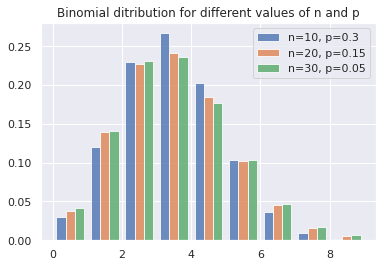
\includegraphics[width=0.5\textwidth]{../../images/binomial-distribution.png}
    \caption{Binomial distribution for different parameters $n$ and $p$.}
    \label{fig:binomial-distribution}
\end{figure}